\documentclass[a4paper,twocolumn]{article}
\usepackage[utf8]{inputenc}
\usepackage{amsmath}
\usepackage{amsfonts}
\usepackage{amssymb}
\usepackage{tikz}
\usepackage{hyperref}
\usepackage{url}
\usepackage{paralist}
\usepackage[left=2cm,right=2cm,top=2cm,bottom=2cm]{geometry}
\RequirePackage[date=terse,isbn=true,doi=true,url=false,maxbibnames=9,backref=false]{biblatex}
\addbibresource{securityupdates.bib}
\renewcommand{\bibfont}{\small}

\AtEveryBibitem{% Clean up the bibtex rather than editing it
 \clearname{editor} % remove editors
}

\author{Daniel Thomas}
\title{Android security updates}
\date{}%no date, it takes up space
\begin{document}
\maketitle

\section*{Problem definition}
Last year I proposed Nigori, a system for secure synchronised storage for Internet of Things devices, this relies on the security of the underlying device and so this year I am proposing looking at the security of the device operating system.

The Internet of Things means that there will be many more internet connected devices, these will have software / firmware running on them.
Security vulnerabilities will be found in this software and firmware which will then need to be updated.
Android is one operating system which is being used for various Internet of Things devices (fridges, toasters etc.) and so examining the trends in security updates for Android gives us insight into how updates for Internet of Things devices might evolve.
Our preliminary results indicate that most Android devices do not receive security updates in a timely manner.
Android devices are user facing and probably more likely to receive updates than fridges or water meters so the situation is likely to be worse.
I intend to quantify this more precisely and compare different manufacturers to determine which are the best at shipping security updates promptly.
Initial analysis indicates that perhaps the Qualcomm Innovation Center, Inc. (QuIC) is the best at following best practice~\cite{codeaurora-security-advisories} and Google the best at shipping updates to devices promptly.


\section*{Innovation proposal and relation to the state of the art}
Presently there is not much visibility into the impact of security vulnerabilities on Android, many root equivalent vulnerabilities do not even have CVEs registered even when they are being actively exploited.
It is also difficult to determine when vulnerabilities have been fixed and these fixes propagated to users.
I have produced the Android Vulnerabilities website~\cite{androidvulnerabilities.org} to collate this information.
Root equivalent vulnerabilities are vulnerabilities which can be exploited either to gain root or to gain privileges which can then be used to gain root on the device.
By using the database of root equivalent vulnerabilities that I have collected and the Device Analyzer~\cite{Wagner2013} data we can determine the proportion of devices running vulnerable versions of Android.
We can then chart how that changes over time as new vulnerabilities are discovered and old ones are fixed, this is shown in Figure \ref{fig:propinsecure}.

\begin{figure}
 \includegraphics[width=0.5\textwidth]{figures/proportioninsecure.pdf}
 \caption{Proportion of devices running vulnerable versions of Android}
 \label{fig:propinsecure}
\end{figure}

There is still much to do, we have only just started.
We need a more representative coverage of root equivalent vulnerabilities on Android, currently we only have a subset with many important details missing from the ones which we have.
In particular manufacturer specific flaws are under-represented and there are many details which need to be tracked down to improve the accuracy of the results.
There is also information which is not presently publicly available but which it might be possible to ask manufacturers and those who found vulnerabilities for in order to get a better picture of what is actually happening.
Presently while we can chart the data we have, we cannot be sure that it is representative.

Existing databases such as the CVE database~\cite{cve-details} lack information vital to performing these sorts of analyses such as dates for discovery, and release dates for fixes.
Even finding release dates for Android versions is difficult as there is no canonical list.
For example dates of tags in the Android Open Source Repository are also unreliable indicators of release dates, sometimes being tagged well after devices have started receiving updates to that version.
Collating all the information together and checking its accuracy is a significant undertaking, the idea is to provide a good starting point and then use crowd-sourcing for the remainder once the Android Vulnerabilities website is a useful resource.
We have already started getting submissions from other people to improve it.

Once we can make accurate comparisons between manufacturers regarding the timeliness with which they ship security updates to customers then we can publish this information and hence create an incentive for manufactures to ship updates more promptly.
CESG which advises government on how to secure its computer system recommends picking Android devices from manufactures which are good at shipping security updates promptly~\cite{CESG2013} but it does not state which manufacturers are better.
Enterprises with Bring Your Own Device (BYOD) policies or which supply smartphones for work purposes are likely to also be interested in this information as if an app can root a phone then any attempt to prevent data leakage are rendered useless.

Figure \ref{fig:da_norm_os} shows the proportion of devices in the Device Analyzer data running different Android OS versions and how that changes with time.
Figure \ref{fig:norm_os_heat} shows the same data in a way which is easier to read when comparing how a particular version has changed with time.
Figure \ref{fig:norm_api_heat} shows how the more coarse grained API version varies.

Figure \ref{fig:propinsecure} shows the proportion of devices running versions of Android with known root vulnerabilities, Figure \ref{fig:nvulnerabilities_heat} breaks this down by vulnerability to show how the proportion of devices affected by different vulnerabilities varies.
It clearly shows how the the APK signing vulnerabilities affected all devices and took a while to get fixed for any device.
However what is perhaps more worrying is the long tail on vulnerabilities such as Gingerbreak, levitator and exploid which are more dangerous root exploits (not requiring new package installation) and which still affect a significant proportion of devices years after they were discovered.

These graphs only show a small subset of the total vulnerabilities and only those which affect all Android devices, not any that are manufacturer or device specific.
Hence observations of the proportion of devices affected in total are underestimates.
\begin{figure}
 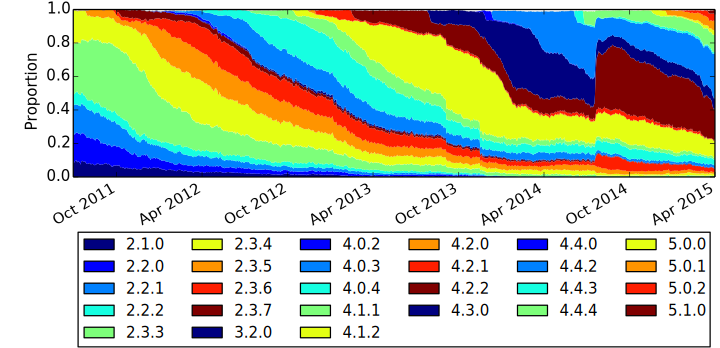
\includegraphics[width=0.5\textwidth]{figures/da_norm_os.pdf}
 \caption{Proportion of devices running different OS versions in the DA data (see also \ref{fig:norm_os_heat})}
 \label{fig:da_norm_os}
\end{figure}
\begin{figure}
 \includegraphics[width=0.5\textwidth]{figures/norm_os_heat.pdf}
 \caption{Proportion of devices running different OS versions in the DA data (see also \ref{fig:da_norm_os})}
 \label{fig:norm_os_heat}
\end{figure}
\begin{figure}
 \includegraphics[width=0.5\textwidth]{figures/norm_api_heat.pdf}
 \caption{Proportion of devices running different API versions in the DA data}
 \label{fig:norm_api_heat}
\end{figure}
\begin{figure}
 \includegraphics[width=0.5\textwidth]{figures/nvulnerabilities_heat.pdf}
 \caption{Proportion of devices affected by different vulnerabilities}
 \label{fig:nvulnerabilities_heat}
\end{figure}

Figure \ref{fig:from_to_updates} shows how devices upgrade between different versions of Android.
Device Analyzer observes upgrade events and the figure shows which versions a device is upgrading from and to.
Mostly the cells with version change are above the diagonal and are upgrades, while many upgrades are from one version to the next version there are also a fair number which skip a few versions.
Surprisingly there are also a small number of downgrade events when older versions of Android are installed on to devices.
Figure \ref{fig:weekly_security_updates} shows the number of devices getting security updates each week, blue shows updates which changed the Android version number from a version with known vulnerabilities to one which had fewer known vulnerabilities.
Red indicates updates which changed the build number but not the version number and so might contain a backported fix for a vulnerability.

\begin{figure}
 \includegraphics[width=0.5\textwidth]{figures/from_to_updates.pdf}
 \caption{Updates between different Android versions in the DA data}
 \label{fig:from_to_updates}
\end{figure}
\begin{figure}
 \includegraphics[width=0.5\textwidth]{figures/w_security_updates.pdf}
 \caption{Number of updates each week which fixed or may have fixed security vulnerabilities}
 \label{fig:weekly_security_updates}
\end{figure}


\section*{One year horizon}
\begin{itemize}
 \item A comprehensive database of root equivalent vulnerabilities affecting Android in a machine readable format on the website~\cite{androidvulnerabilities.org}.
 \item Comparison of different manufacturers to determine which is best at shipping updates for security vulnerabilities.
 \item Analysis of the behaviour of users with respect to Android updates -- how promptly do they get installed once made available.
 \item What else???
\end{itemize}


\section*{Conclusion}
We have collected some data on root equivalent vulnerabilities on Android and version information for deployed Android devices.
Preliminary results are interesting and with more and better data we should be able to make useful recommendations about which manufacturers are best at shipping security updates.
This in turn should incentivise manufactures to do a better job and so improve end user security.
Improvements in end user security should give users more confidence in using their devices and this confidence is vital if the Internet of Things is to work out.
We will hopefully also be able to analyse the incentives which have created the current situation and look at how those could be changed.


\printbibliography

\end{document}